\chapter{Methods}

\section{Study Design}
\subsection{Prospective or retrospective study}
((Prospective or retrospective study)) \\


One important property of CNNs is the “transferability”. Due to the efforts of the doctors in NTUH, we have sufficiently large pancreatic dataset. We want to use this precious data to help train models for other pancreatic dataset. It deeply relies on the "transferability” of CNN, in other words, transfer-learning. 

But there are multiple transfer-learning methods, why we choose fine-tuning? According to this thesis Learning without Forgetting \cite{li2017learning}, the authors compare four methods, including joint training, feature extraction, learning without forgetting and  fine-tuning. The fine-tuning method performs well in external data, and also has excellent testing efficiency. Another thesis in 2017 applies fine-tuning on ultrasound images and has an obvious enhance on model performance. \cite{chi2017thyroid}

Since 2018, our team continues collecting new external data and labeling the images. If we can select patient data that provides information most, the model performance increases more for certain amounts of labeled data. \cite{zhou2017fine} provides AIFT method to do data selection. 

The thesis applies fine-tuning model on pancreatic images, also data selection will be applied. 

\subsection{Study goal*}
((Study goal, such as model creation, exploratory study, feasibility study, noninferiority trial)) \\
\section{Data}
\subsection{Data Source}
((Data sources)) \\
This thesis applies three datasets. All of them are pancreatic CT images.
\begin{itemize}
    \item {\bf National Taiwan University Hospital (ntuh, source data)} \\including both healthy(400) and tumor(400) CT scans. 
    \item {\bf Medical Segmentation Decathlon\cite{simpson2019large} (msd, target data)}\\ including only tumor(281) CT scans. 
    \item {\bf The Cancer Imaging Archive (tcia, target data)}\\ including only healthy(82) CT scans. 
\end{itemize}

\subsection{Eligibility criteria*}
((Eligibility criteria: how, where, and when potentially eligible participants or studies were identified (eg,
symptoms, results from previous tests, inclusion in registry, patient-care setting, location, dates))) \\

\subsection{Data Preprocessing}
((Data preprocessing steps)) \\
All CT images that contained the pancreas or PC from an individual subject were manually labeled for further model training/validation and testing using an open source software (3D Slicer version 4.8.1). 
Since the pancreas bordered multiple organs/structures and PCs often had an indistinct border with the surrounding tissue, there are inter-observer differences regarding the exact extent of the pancreas and the cancer tumor. Therefore, the labeled pancreas and tumor on the images were checked by the radiologists before further processing and analysis steps. The window width and window level were fixed as 250 Hounsfield unit (HU) and 75 HU, respectively. The images were normalized to [0, 1] by linear interpolation, and the portions that were neither pancreas nor tumor were excluded from further analysis. The images were then cropped into square sub-regions (i.e. 50 X 50 patches) using the moving window method on the axial (x-y) plane, starting from the top-left corner and ended at the bottom-right corner. Moving distance was set as half of the patch dimension to generate overlapping patches in order to increase the variation and size of training data. The patches which contained PC were labeled as cancerous, whereas patches that contained only non-cancerous pancreatic parenchyma were labeled as non-cancerous.

\subsection{Selection of data subsets(ignore)}
((Selection of data subsets, if applicable(ignore)))
\subsection{Definitions of data elements(ignore)}
((Definitions of data elements, with references to common data elements(ignore)))
\subsection{De-identification Methods*}
((De-identification methods))
\subsection{Missing Data*}
((How missing data were handled(ignore)))



\section{Ground Truth*}
\subsection{Reference Standard}
((Definition of ground truth reference standard, in sufficient detail to allow replication))
\subsection{Rationale for choosing the reference standard}
((Rationale for choosing the reference standard (if alternatives exist))) \\
\subsection{Source of Ground Truth Annotations}
((Source of ground truth annotations; qualifications and preparation of annotators)) \\
\subsection{Annotation tools}
((Annotation tools)) \\
\subsection{Measurement of inter and intrarater variability}
((Measurement of inter and intrarater variability; methods to mitigate variability and/or resolve discrepancies)) \\



\section{Data Partitions*}
\subsection{Sample Size and How It Was Determined}
((Intended sample size and how it was determined))
\subsection{Assign to partitions}
((How data were assigned to partitions; specify proportions))


\section{Model}
\subsection{Detailed description of model}
((Detailed description of model, including inputs, outputs, all intermediate layers and connections)) \\

The CNN model was modified from VGG network12, a neural network widely used in image classification. Weighted binary cross-entropy13 was used as the loss function to solve the  imbalance problem between the number of cancerous and noncancerous patches. Table 1 provides the details of the CNN model, including the layer structures, kernel sizes, channels, and output sizes of the network.
Two callbacks monitoring on validation loss were used during the training process to optimize model performance. All codes were written in Python (version 3.6.8) using Keras (version 2.2.4)14 and Tensorflow (version 1.7.0)15 libraries.

\begin{table}[H]
\centering
\caption{CNN model Structure}
\begin{tabular}{|l|l|l|} 
\hline
Layer (type)              & Output Shape      & Parameter  \\ 
\hline
conv2d 1 (Conv2D)             & (None, 50, 50, 16) &  416 \\
\hline
conv2d 2 (Conv2D)        & (None, 50, 50, 32)                        & 12832        \\
\hline
max pooling2d 1 (MaxPooling2) &  (None, 50, 50, 32) &  0         \\
\hline
conv2d 3 (Conv2D)                                    & (None, 25, 25, 64)                        & 18496                            \\
\hline
conv2d 4 (Conv2D)             & (None, 25, 25, 64) & 36928     \\
\hline
max pooling2d 2 (MaxPooling2)                        & (None, 12, 12, 64)                        & 0                                \\
\hline
conv2d 5 (Conv2D)                                    & (None, 12, 12, 128)                       & 73856                            \\
\hline
conv2d 6 (Conv2D)                                    & (None, 12, 12, 128)                       & 147584                           \\
\hline
max pooling2d 3 (MaxPooling2)                        & (None, 6, 6, 128)                         & 0                                \\
\hline
flatten 1 (Flatten)                                  & (None, 4608)                              & 0                                \\
\hline
dense 1 (Dense)                                      & (None, 32)                                & 147488                           \\
\hline
dropout 1 (Dropout)                                  & (None, 32)                                & 0                                \\
\hline
dense 2 (Dense)                                      & (None, 32)                                & 1056                             \\
\hline
dense 3 (Dense)                                      & (None, 1)                                 & 33 \\
\hline
\end{tabular}
\end{table}

\subsection{Software libraries, frameworks, and packages*}
((Software libraries, frameworks, and packages)) \\
\subsection{Initialization of model parameters*}
((Initialization of model parameters (eg, randomization, transfer learning))) \\



\section{Training*}
\subsection{Training approach}
((Details of training approach, including data augmentation, hyperparameters, number of models trained)) \\
\subsection{Method of selecting the final model}
((Method of selecting the final model)) \\
\subsection{Ensembling techniques, if applicable(ignore)}
((Ensembling techniques, if applicable(ignore))) \\

\section{Evaluation}
This chapter consists of three experiments: basic validation, mix data training and fine tuning. To better observing the result, this thesis use cross validation to distribute training/validation/testing set. 


\subsection{Model performance}
((Metrics of model performance)) \\

\subsubsection{Basic Validation}
In this part, we train model only using target data. We want to find how many patients in target data is needed to build a sufficiently nice model. That means, the AUC of model is larger than 0.8. The table below is the diagram of the number of training/validation/testing set of this experiment. We increase the number of target data to observe the performance of model trained by target data (82, 164, 246, 326 target data).
\begin{table}[H]
\centering
\caption{training/validation/testing set (A) (Basic Validation, 10 folder)}
\begin{tabular}{|l|l|l|l|l|} 
\hline
~            & source H & source T & target H (tcia) & target T (msd)  \\ 
\hline
train        & 0      & 0      & -               & -               \\ 
\hline
validation   & 0       & 0       & -               & -               \\ 
\hline
source test  & 40       & 40       & 0               & 0               \\ 
\hline
target test~ & 0        & 0        & 8               & 28              \\
\hline
\end{tabular}
\end{table}

\begin{table}[H]
\centering
\caption{training/validation/testing set (B) (10 folder)}
\begin{tabular}{|l|l|l|l|l|} 
\hline
amount of data   & tar H (train) & tar T (train) & tar H (val) & tar T (val)  \\ 
\hline
82        & 17      & 57      & 2               & 6               \\ 
\hline
164   & 33       & 114       & 4               & 13               \\ 
\hline
246  & 50       & 171       & 6               & 19               \\ 
\hline
326 & 66        & 228        & 7               & 25              \\
\hline
\end{tabular}
\end{table}

\subsubsection{Mix Source and Target Data}
In this part, we train model using both source data and target data. We want to find how the number of  patients in target data influences the model performance. The table below is the diagram of the number of training/validation/testing set of this experiment. We increase the number of target data to observe the performance of joint training (82, 164, 246, 326 target data).

\begin{table}[H]
\centering
\caption{training/validation/testing set (Mix Source and Target Data)}
\begin{tabular}{|l|l|l|l|l|} 
\hline
~            & source H & source T & target H (tcia) & target T (msd)  \\ 
\hline
train        & 324      & 324      & -               & -               \\ 
\hline
validation   & 36       & 36       & -               & -               \\ 
\hline
source test  & 40       & 40       & 0               & 0               \\ 
\hline
target test~ & 0        & 0        & 8               & 28              \\
\hline
\end{tabular}
\end{table}

\subsubsection{Transfer Learning}
In this part, first we train model only using source data. Than I use the weight of the previous model as the initial value of training. I train the previous model again using target. The table below is the diagram of the number of training/ validation/ testing set of this experiment. 

\begin{table}[H]
\centering
\caption{training/validation/testing set (A) (Basic Validation, 10 folder)}
\begin{tabular}{|l|l|l|l|l|} 
\hline
~            & source H & source T & target H (tcia) & target T (msd)  \\ 
\hline
train        & 0      & 0      & -               & -               \\ 
\hline
validation   & 0       & 0       & -               & -               \\ 
\hline
source test  & 40       & 40       & 0               & 0               \\ 
\hline
target test~ & 0        & 0        & 8               & 28              \\
\hline
\end{tabular}
\end{table}

\begin{table}[H]
\centering
\caption{training/validation/testing set (B) (10 folder)}
\begin{tabular}{|l|l|l|l|l|} 
\hline
amount of data   & tar H (train) & tar T (train) & tar H (val) & tar T (val)  \\ 
\hline
82        & 17      & 57      & 2               & 6               \\ 
\hline
164   & 33       & 114       & 4               & 13               \\ 
\hline
246  & 50       & 171       & 6               & 19               \\ 
\hline
326 & 66        & 228        & 7               & 25              \\
\hline
\end{tabular}
\end{table}

\subsection{Statistical measures of significance and uncertainty*}
((Statistical measures of significance and uncertainty (eg, confidence intervals))) \\
\subsection{Robustness or sensitivity analysis*}
((Robustness or sensitivity analysis)) \\
\subsection{Methods for explainability or interpretability*}
((Methods for explainability or interpretability (eg, saliency maps) and how they were validated)) \\
\subsection{Validation or testing on external data(ignore)}
((Validation or testing on external data(ignore))) \\





\subsection{Area under the Receiver Operating Characteristic Curve (AUC)?}
A receiver operating characteristic curve, or ROC curve, is a graphical plot that shows the diagnostic ability of a binary classifier system as its predict threshold is varied. The area under the receiver operating characteristic curve is a common criteria to evaluate model performance, not depending on patient threshold. We use AUC in our this thesis. 


\subsection{Transfer Learning and Fine-Tuning?}
In real-world applications, the assumption that the training and future data must be in the same feature space and have the same distribution may not hold. In such cases, knowledge transfer, if done successfully, would highly improve the performance of learning by avoiding much expensive data-labeling efforts. In medical image research, patient data and label is precious and hard to get. Transfer learning has emerged as a new learning framework to solve this problem. Since the target data is labeled, the thesis use fine-tuning to enhance the prediction performance.\cite{pan2009survey}

\subsection{Cross Validation?}
Cross-validation is any of various similar model validation techniques for assessing how the results of a model will generalize to an independent data set.One wants to estimate how accurately a predictive model will perform in practice. The goal of cross-validation is to test the model's ability to predict new data that was excluded from training data, in order to deal with problems like overfitting or selection bias.
\\
Take 5-folder cross validation as an example. There are 400 healthy ntuh data. First we split it into 5 groups (80 data for each group) and take them as test set. 90 percent of the remained data is the training data while 10 percent is the validation data. (Figure 3.1)

\begin{figure}[H]
    \hfil
    \begin{minipage}[t]{0.9\textwidth}
        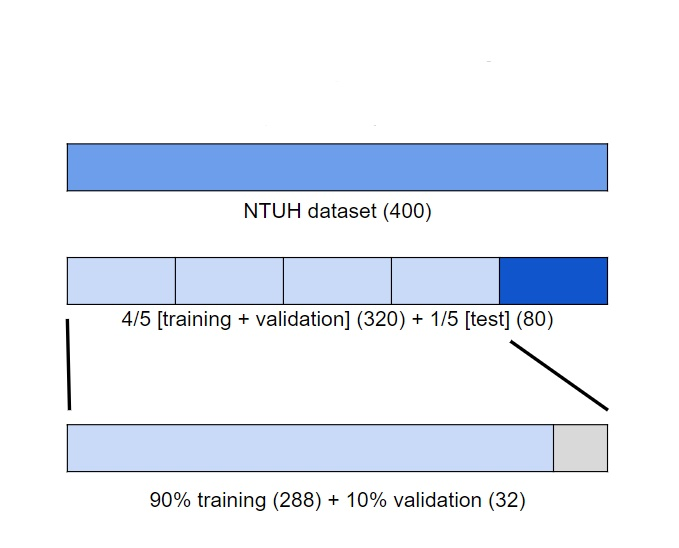
\includegraphics[width=\textwidth]{fig/cross.png}
        \caption{\label{fig:parallel1} training/validation/testing set distribution}
    \end{minipage}
    \hfil
\end{figure}


